\documentclass[t,xcolor={usenames,dvipsnames}]{beamer}

\mode<presentation>
{
\usetheme{Frankfurt}
}

\usepackage[english]{babel}
\usepackage[latin1]{inputenc}
\usepackage{times}
\usepackage[T1]{fontenc}
\usepackage{verbatim}
\usepackage{url}
\usepackage{amsmath,amssymb}
\usepackage{comment}
\usepackage{hyperref}

% Author-date citations
\usepackage[authoryear,round]{natbib}
\let\cite=\citep  % default \cite such as {\LaTeX} authors are used to

% Where \includegraphics should look for figures
\graphicspath{{./figs/}}
\usepackage{epstopdf}
\DeclareGraphicsExtensions{.eps,.png,.jpg,.pdf}

% Shortcuts
\newcommand{\myhref}[2]{\href{#1}{\textcolor{Blue}{#2}}}
\newcommand{\myurl}[1]{\myhref{#1}{#1}}
\newcommand{\subitem}[1]{\begin{itemize}[<.->]\item #1 \end{itemize}}
\newcommand{\ghead}[1]{{\tiny #1\\}}
\newcommand{\doi}[1]{\myhref{http://dx.doi.org/#1}{doi:#1}}
\newcommand{\csym}[1]{\textcolor{Blue}{\texttt{#1}}}


%%%%%%%%%%%%%%%%%%%%%%%%%%%%%%%%%%%%%%%%%%%%%%%%%%%%%%%%%%%%%%%%%%%%%%
\title{Cardiac Electrophysiology Web Lab}
\author{Jonathan Cooper \& Gary Mirams}
\institute[University of Oxford]
{Computational Biology Group\\
 Department of Computer Science\\
 University of Oxford}
\date{13\textsuperscript{th} March 2015}

\begin{document}

\begin{frame}
\titlepage
\end{frame}

%%%%%%%%%%%%%%%%%%%%%%%%%%%%%%%%%%%%%%%%%%%%%%%%%%%%%%%%%%%%%%%%%%%%%%

%\begin{frame}{Outline}
%\setcounter{tocdepth}{1}
%\tableofcontents
%\end{frame}

%%%%%%%%%%%%%%%%%%%%%%%%%%%%%%%%%%%%%%%%%%%%%%%%%%%%%%%%%%%%%%%%%%%%%%
\section{Introduction}
\subsection*{Main}
%%%%%%%%%%%%%%%%%%%%%%%%%%%%%%%%%%%%%%%%%%%%%%%%%%%%%%%%%%%%%%%%%%%%%%
% Brief intro to FC, focus on sell & concept

\begin{frame}{Improving the process of modelling}
\begin{itemize}[<2>]
\item As hypothesis encodings, models are developed \emph{for a specific purpose}
  \subitem{May not be appropriate for studying same system in different context}
\item How can we\ldots
  \begin{itemize}
  \item determine a model's functionality, i.e.\ its suitability or limitations for a new study? % Perhaps as part of a composite
  \item re-use a model in a different experimental context?
  \item compare hypotheses: different models' behaviours under the same experiment?
  \end{itemize}
\end{itemize}
\end{frame}


\begin{frame}{Functional curation with virtual experiments}
\vspace{-.2cm}
\subitem{Separate \alert{model structure} and \alert{experimental scenario}}
\vspace{-.2cm}
\hspace{-1cm}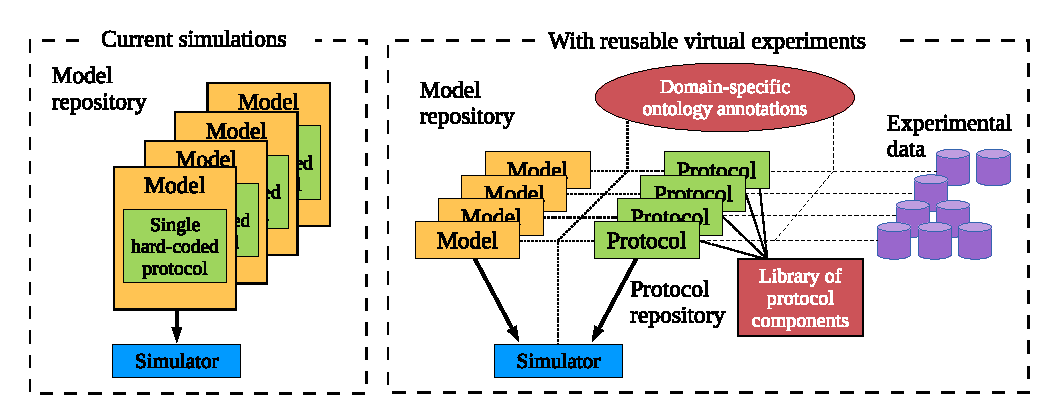
\includegraphics[width=1.185\textwidth]{virtual_expts_schematic}
\vspace{-.31cm}
\begin{itemize}
\item Apply any \alert{virtual experiment} to any (relevant) model
\item One definitive version of each model / protocol
\item Automatically generate post-processed outputs, plots, etc.
\end{itemize}
\end{frame}


\begin{frame}{Exemplar system: Cardiac electrophysiology}
\begin{center}
\vspace{-.5cm}
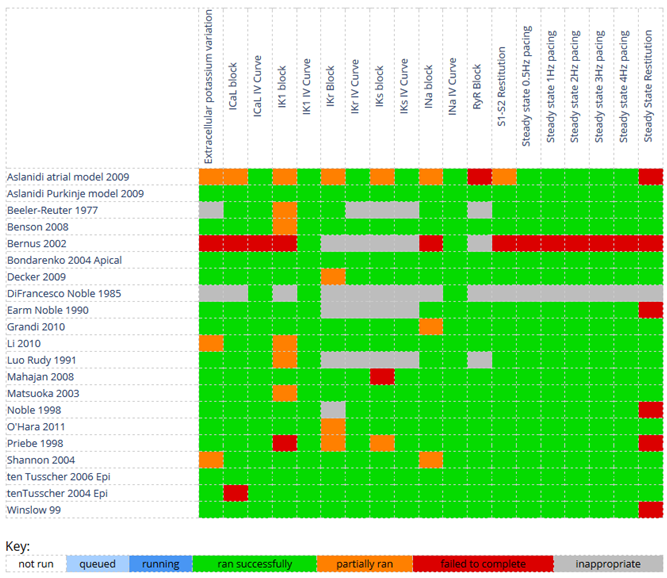
\includegraphics[height=.8\textheight]{cardiac_fc_matrix}\\
\myurl{https://chaste.cs.ox.ac.uk/FunctionalCuration}
\end{center}
\end{frame}

%%%%%%%%%%%%%%%%%%%%%%%%%%%%%%%%%%%%%%%%%%%%%%%%%%%%%%%%%%%%%%%%%%%%%%
\section{Sample results}
\subsection*{Main}
%%%%%%%%%%%%%%%%%%%%%%%%%%%%%%%%%%%%%%%%%%%%%%%%%%%%%%%%%%%%%%%%%%%%%%

\begin{comment}
Ideally this section will be done as a live demo, and the slides skipped
(except possibly the last one, which is harder to show live).
But if that fails you can talk about these examples.

Start by going to the main experiments matrix, select regular 2 Hz pacing, and compare all models.
Back to main matrix, compare mode, select just human models, compare 2 Hz pacing.
Show sub-matrix for human models.
	Compare both restitution protocols for all human models.
	Compare drug block for different models: IKr then NCX.
	On IKr, show the detailed results for O'Hara to demonstrate why it's missing a point for 100% block.
	Compare extracellular K+.
Show use in fixing models: view the Decker model, show version table, compare with BiVeS.
	Have https://chaste.cs.ox.ac.uk/q/2014/fc/s1s2 in separate tab as hard to browse to!
	Note that BiVeS is Martin's PhD work - the intern who first developed the Web Lab.
Show metadata annotation
	View your files, pick a model, and click the edit metadata link
	Talk about what can do, and mention plans to structure the metadata ontology (classify tags by type, show tags used by protocols, tags used by Chaste, etc.)
\end{comment}

\begin{frame}{Results: regular pacing}
\begin{center}
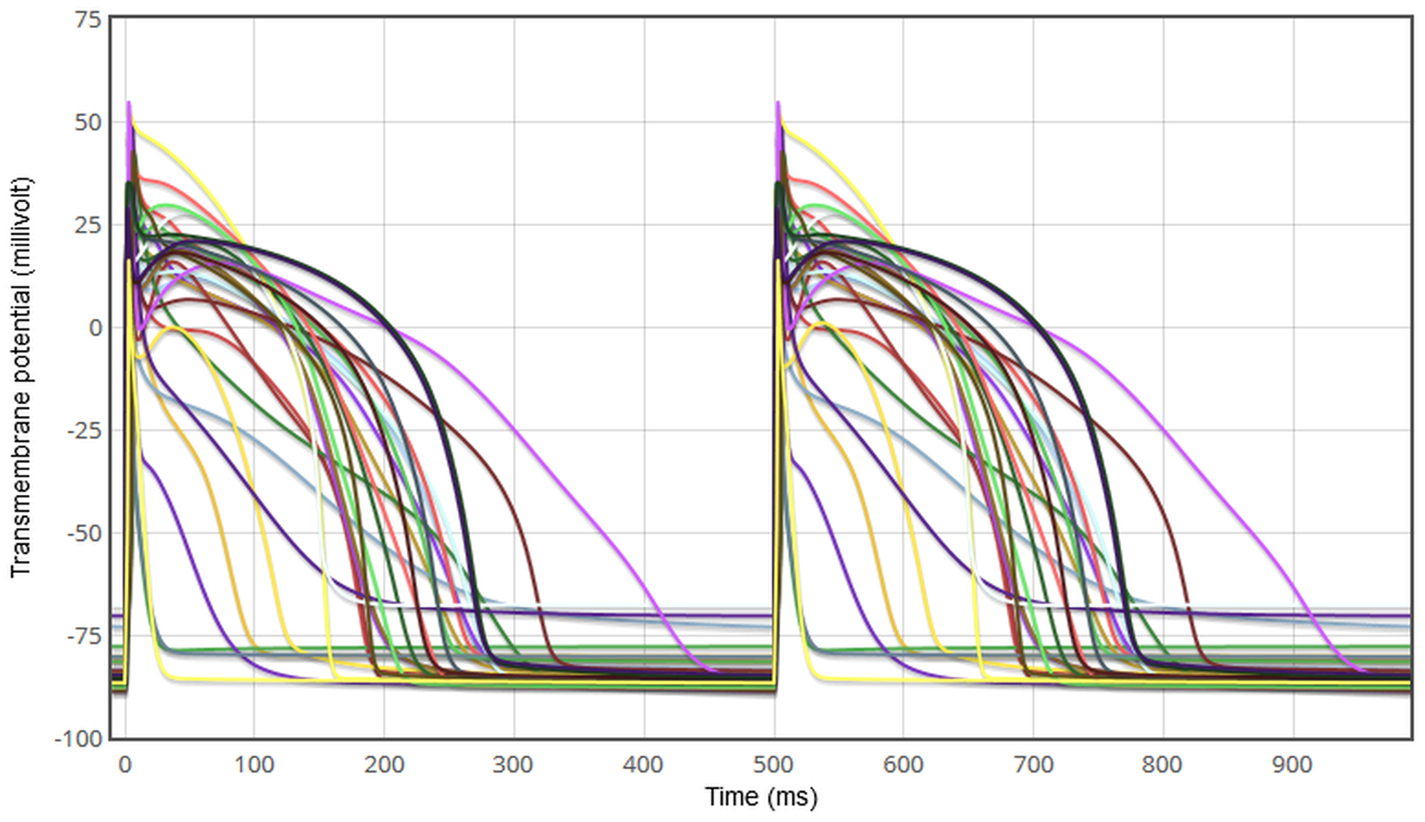
\includegraphics[width=\textwidth]{weblab_fig3}\\
\tiny\myurl{https://chaste.cs.ox.ac.uk/q/2014/fc/fig3}
\end{center}
\end{frame}


\begin{frame}{Results: restitution}
\begin{center}
\vspace{-.5cm}
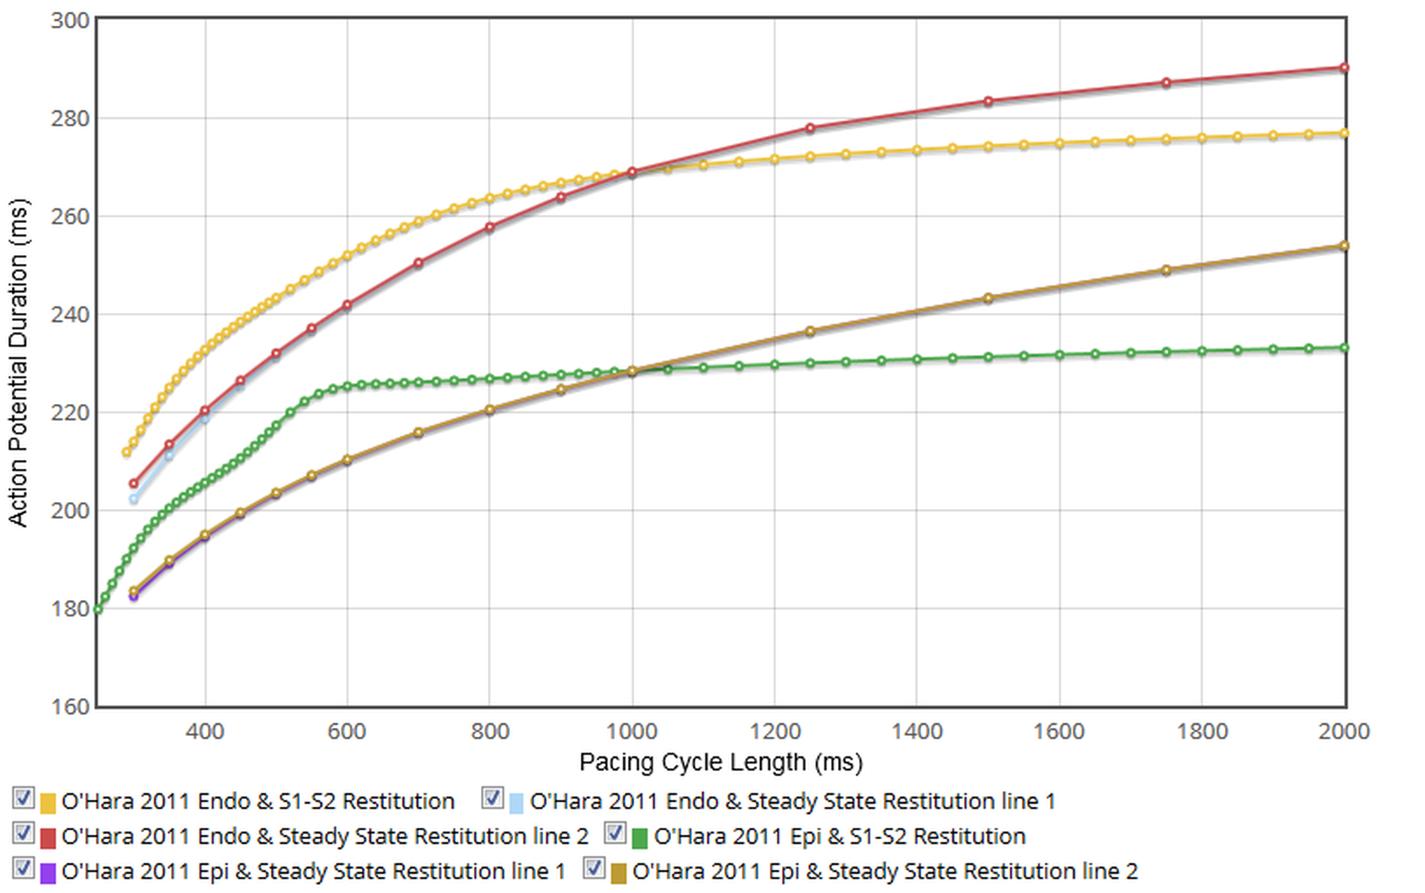
\includegraphics[width=\textwidth]{weblab_fig4}\\
\tiny\myurl{https://chaste.cs.ox.ac.uk/q/2014/fc/fig4}
\end{center}
\end{frame}


\begin{frame}{Results: drug block of IKr}
\begin{center}
\vspace{-.5cm}
\includegraphics[width=\textwidth]<1>{human_ikr_block}
\includegraphics[width=\textwidth]<2>{ohara_endo_ikr_block}
\end{center}
\end{frame}


\begin{frame}{Results: drug block of NCX}
\begin{center}
\vspace{-.5cm}
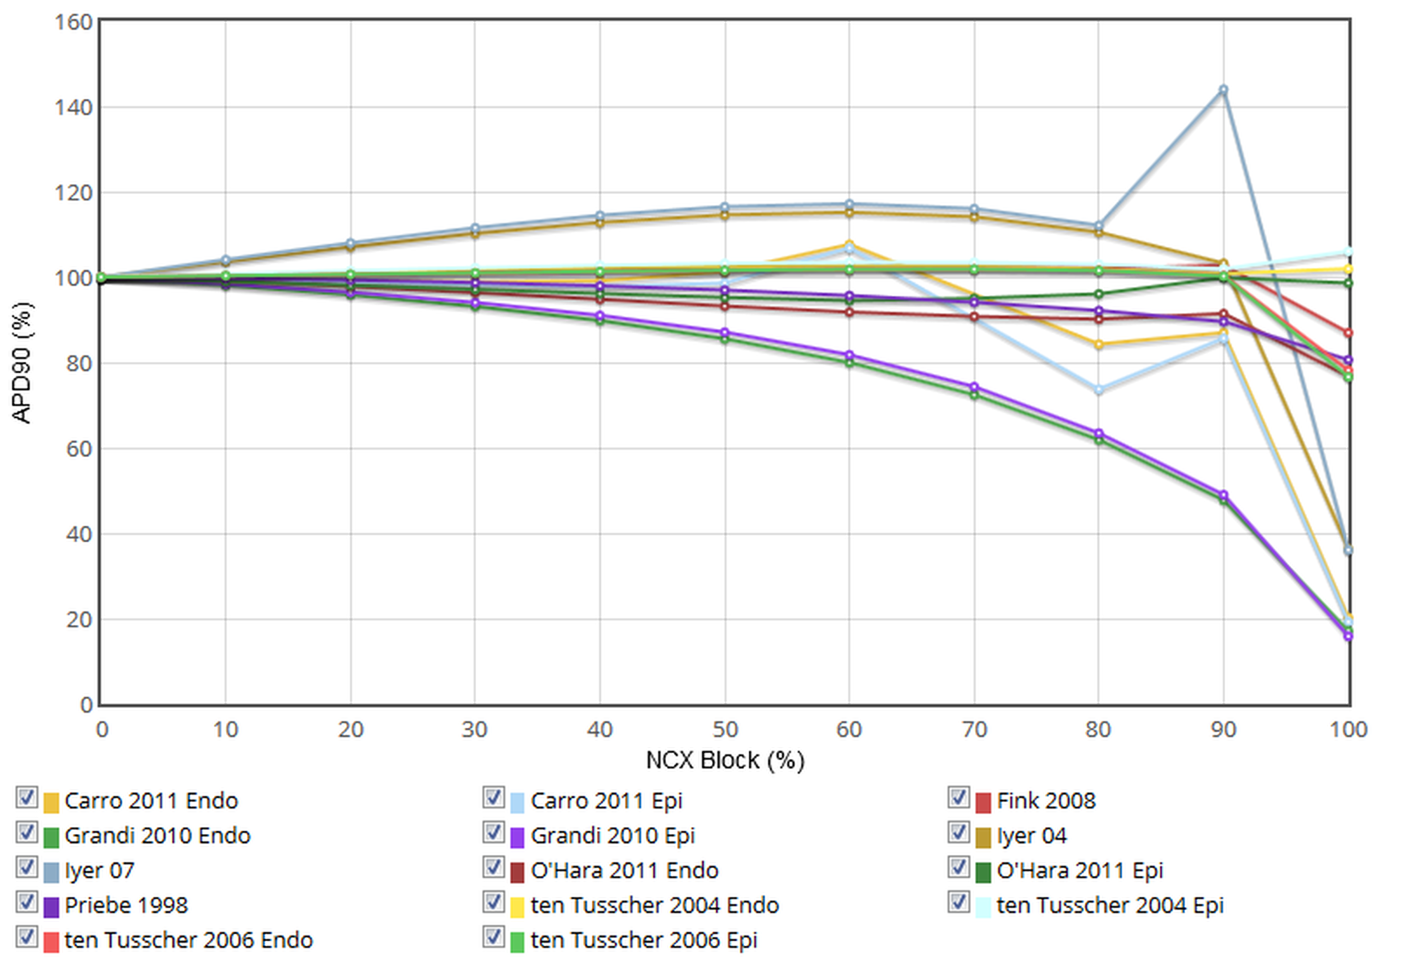
\includegraphics[width=\textwidth]{weblab_fig5}\\
\tiny\myurl{https://chaste.cs.ox.ac.uk/q/2014/fc/fig5}
\end{center}
\end{frame}


\begin{frame}{Results: effects of cell environment}
\begin{center}
\vspace{-.5cm}
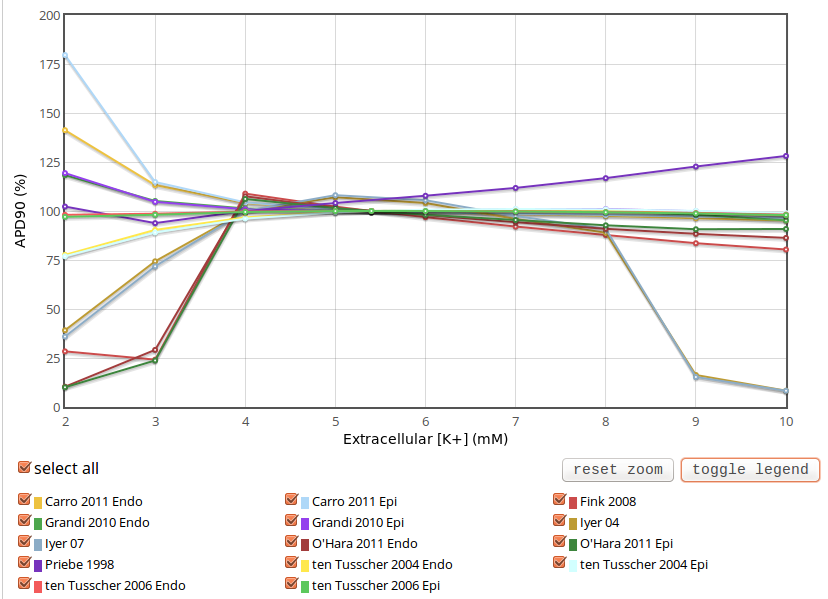
\includegraphics[width=\textwidth]{weblab_extra_K}
\end{center}
\end{frame}


\begin{frame}{Results: fixing model encodings}
\begin{center}
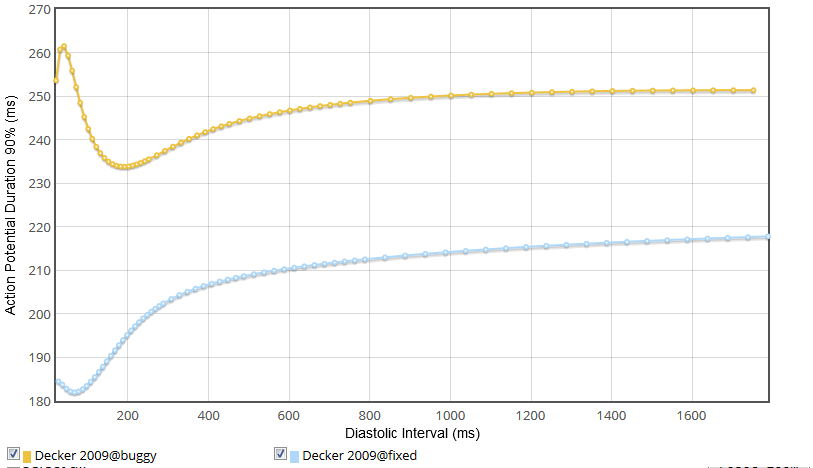
\includegraphics[width=\textwidth]{decker_comparison}

\tiny
\myurl{https://chaste.cs.ox.ac.uk/q/2014/fc/s1s2}

\myurl{https://chaste.cs.ox.ac.uk/q/2014/fc/diff}
\end{center}
\end{frame}


\begin{frame}{Results: steady state behaviour}
Priebe model under drug block of $I_{K_r}$.\\
\textbf{Left}: after just one pace at each degree of IKr block, these results are the same as those shown in Priebe et al. 1998.\\
\textbf{Right}: after 10000 paces for each degree of IKr block as shown in the Web Lab. Note that even the control action potential varies considerably, and is much longer in the steady state case.
\begin{center}
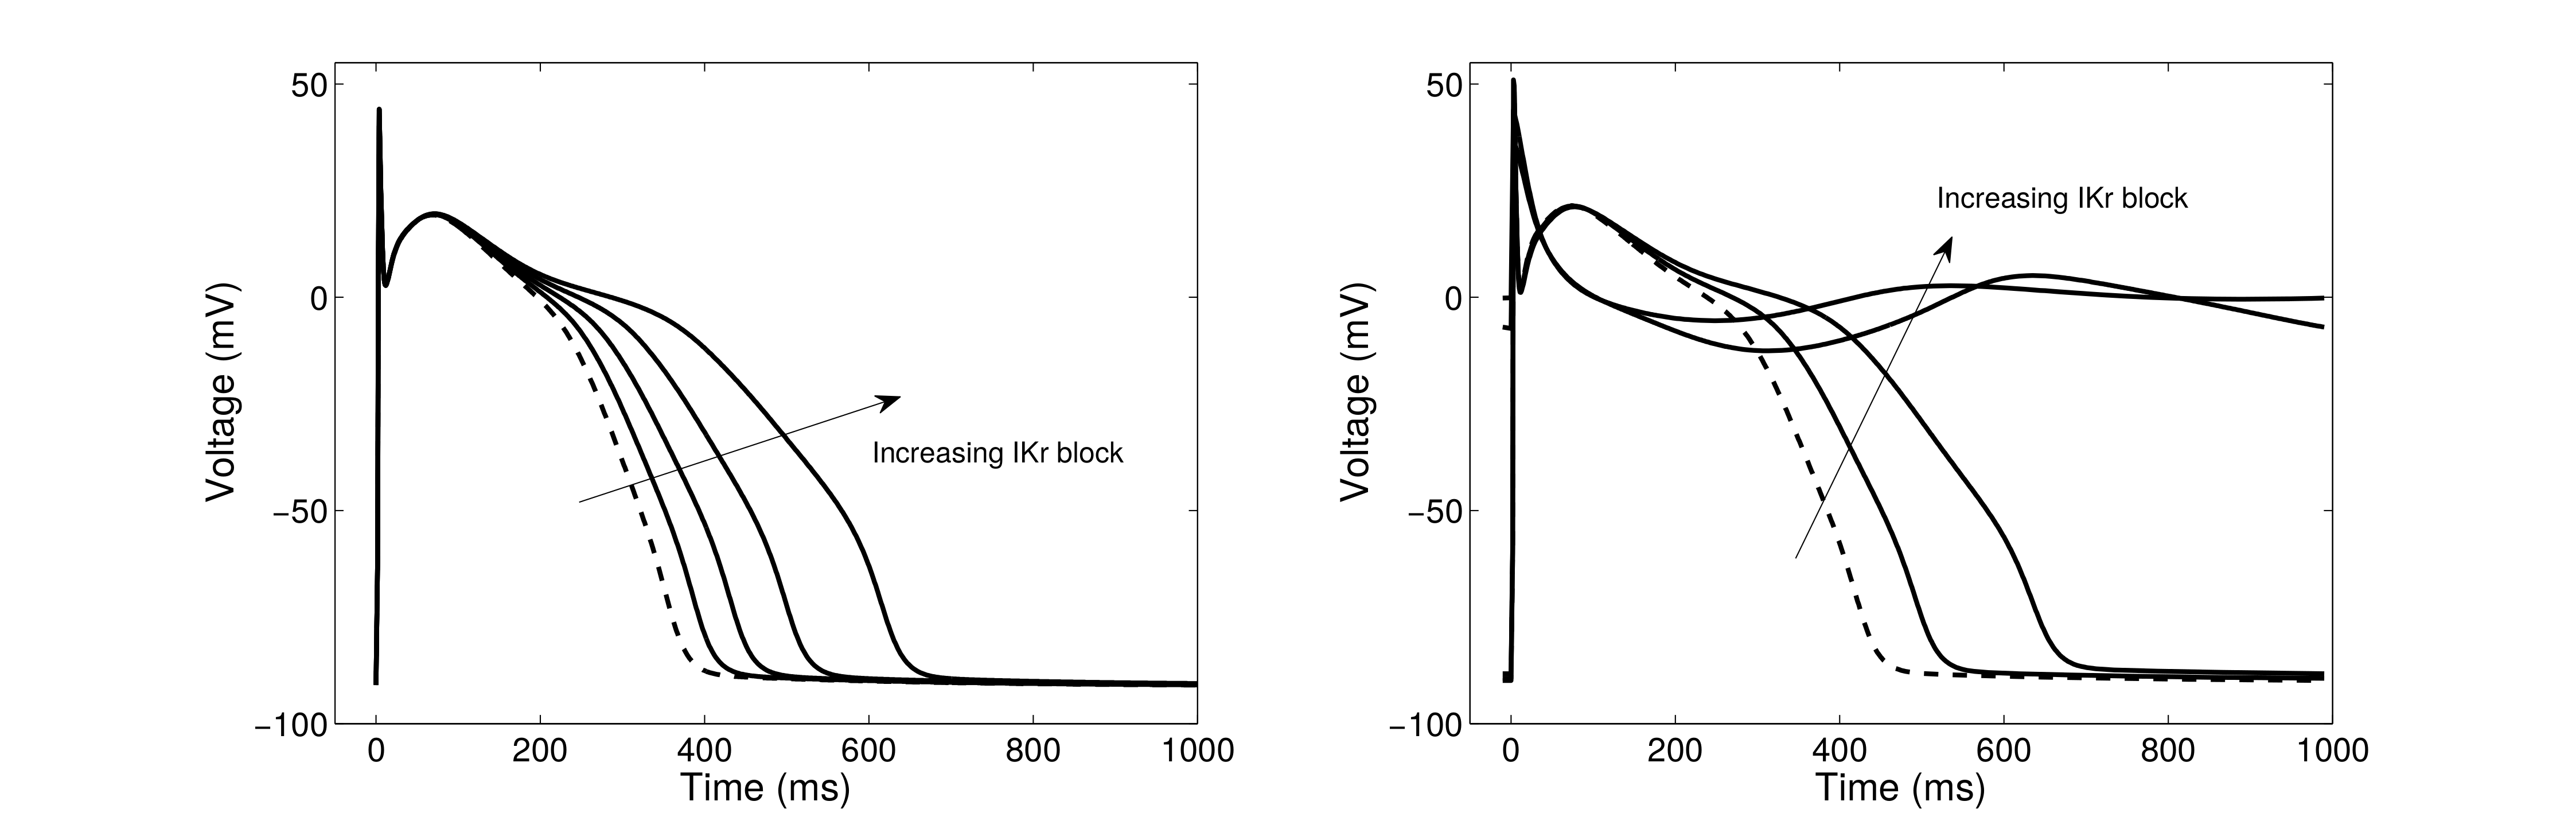
\includegraphics[width=\textwidth]{weblab_fig6}
\end{center}
\end{frame}

%%%%%%%%%%%%%%%%%%%%%%%%%%%%%%%%%%%%%%%%%%%%%%%%%%%%%%%%%%%%%%%%%%%%%%
\section{Perspective and plans}
\subsection*{Main}
%%%%%%%%%%%%%%%%%%%%%%%%%%%%%%%%%%%%%%%%%%%%%%%%%%%%%%%%%%%%%%%%%%%%%%

\begin{frame}{What about reproducibility?}
Or, can you trust the results?
\begin{itemize}
\item The Web Lab stores all previously generated results
\item You can compare with previous versions of models, protocols and/or software
\item This isn't automatic
\item Separate test of the Chaste backend does automated regression testing of software, using a subset of the models and protocols
\end{itemize}
\end{frame}


\begin{frame}{Engagement and outreach}
\begin{itemize}
\item Paper submitted to high profile cardiac journal (Circ Res)
\item Workshop being planned for September 2015
\item Highlighting to our contacts
\end{itemize}
\end{frame}


\begin{frame}{Future plans}
\begin{itemize}
\item Further improvements to ease of use
  \begin{itemize}
  \item Especially for writing new protocols
  \item Better documentation
  \item More flexibility in the language
  \item Allow exploratory investigation of data?
  \end{itemize}
\item More structure in ontology
\item Explicit link to experimental data --- parameter fitting
\end{itemize}
\only<2>{
Longer term\ldots
\begin{itemize}
\item Cloud-based service
\item Integration with best-of-breed repositories for models and experimental data
  \subitem{Key for longevity and embedding within daily life}
\end{itemize}}
\end{frame}


\begin{frame}{Python re-implementation: motivations}
The Web Lab backend is (mostly) C++ simulation code built on Chaste.\\
This is being re-implemented in Python.

\begin{itemize}[<2>]
\item Make it easier to extend what protocols can do
  \subitem{Especially more flexible post-processing and data structures}
\item Provide a basis for Aidan's parameter fitting work
\item Improve performance !
\end{itemize}
\end{frame}




%%%%%%%%%%%%%%%%%%%%%%%%%%%%%%%%%%%%%%%%%%%%%%%%%%%%%%%%%%%%%%%%%%%%%%
\begin{frame}{Acknowledgments}
Aidan Daly, Chaste team\\

Web Lab: \myurl{https://chaste.cs.ox.ac.uk/FunctionalCuration}

\begin{center}

\includegraphics[scale=.9]{chaste-266x60}\\ \vspace{.3cm}

\includegraphics[scale=.7]{logo2020science}\\ \vspace{.4cm}

\includegraphics[width=.55\textwidth]{EPSRC1RGBLO} \hspace{.1cm}

\includegraphics[scale=.55]{logo_msr}
\end{center}
\end{frame}

\end{document}
